\chapter{Capitolo 3: Albero Evolutivo}
Una delle sfide più importanti della bioinformatica, nonché l'obiettivo principale della filogenetica, è la costruzione degli alberi evolutivi.
\newline
Ricordando la definizione di albero, ovvero un grafo non orientato connesso e aciclico \cite{algoritmiEStruttureDati2}, \textit{L'albero evolutivo} o \textit{albero filogenetico} è un diagramma che rappresenta le relazioni evolutive tra i vari organismi \cite{buildingaphylogenictree}. La sua peculiarità consiste nel poterli costruire in base a dati genetici, genomici o morfologici, affinché si possano descrivere le relazioni che vi sono tra organismi viventi oppure tra specie estinte e specie viventi.
\newline
Gli alberi evolutivi possono essere suddivisi in due categorie: alberi radicati e non radicati.


\section{Albero radicato}
\begin{figure}[h!]
	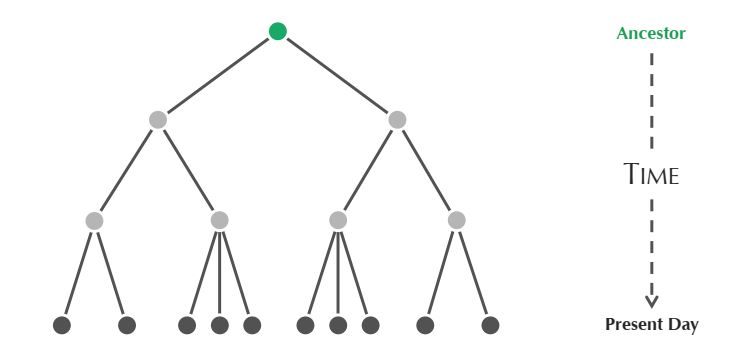
\includegraphics[width=\linewidth]{rooted_tree.jpg}
 	\caption{Un esempio di albero radicato.}
  	\label{fig:RootedTree}
\end{figure}
\textit{L'albero radicato} o \textit{albero con radice} è un albero in cui i nodi rappresentano gli organismi (animali, piante, virus, ecc...), mentre gli archi rappresentano la loro evoluzione nel tempo (figura 2) \cite{bioinfalganactivelearningapproachparttwo}. Esso si sviluppa a partire da un nodo speciale, chiamato \textit{radice} (il vertice verde nella figura) e si estende fino alle foglie. I vertici (o nodi) che hanno grado\footnote{Il grado di un vertice \textit{v} è dato dal numero degli archi incidenti su \textit{v} \cite{algoritmiEStruttureDati2}.} maggiore di uno, definiti \textit{nodi interni}, sono gli antenati, mentre quelli con grado esattamente uguale ad uno, definite \textit{foglie}, sono le forme di vita attualmente esistenti. La radice, quindi, è l'antenato comune a tutti i vertici presenti nell'albero.
\newline
Tale albero con radice non viene usato solamente per conoscere la radice, ma anche per capire quali organismi sono più legati tra loro rispetto ad altri.
\newline
\begin{figure}[h!]
	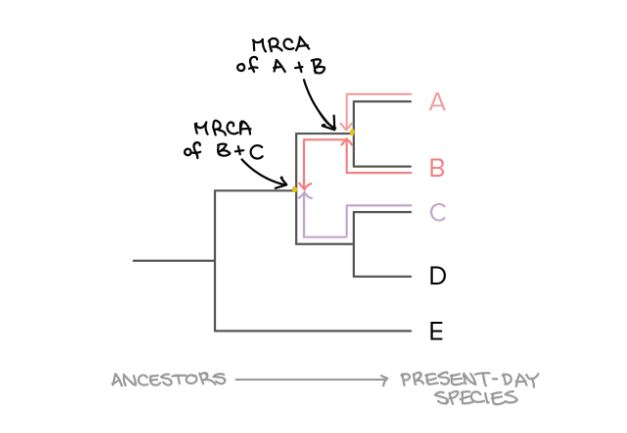
\includegraphics[width=\linewidth]{rooted_tree_2.jpg}
 	\caption{Un esempio di albero radicato che mostra le relazioni tra gli organismi.}
  	\label{fig:RootedTree}
\end{figure}
\newline
Come mostrato nella figura 3, due organismi risultano più legati tra loro se hanno l'antenato più recente in comune ad esempio l'organismo A è più legato a B piuttsto che a C. La sigla "MRCA", infatti, indica il Most Recent Common Ancestor.
\newline
Nei casi in cui non è presente la radice, si parla di albero non radicato.


\section{Albero non radicato}
\begin{figure}[h!]
	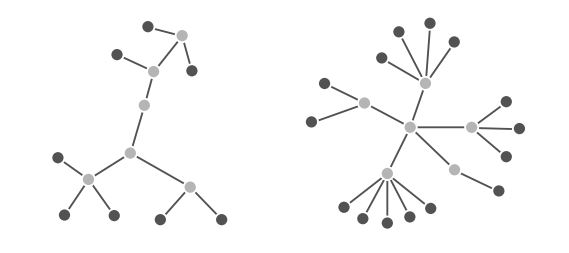
\includegraphics[width=\linewidth]{unrooted_trees.jpg}
 	\caption{Esempi di alberi non radicati.}
  	\label{fig:RootedTree}
\end{figure}
\textit{L'albero non radicato} o \textit{albero senza radice} è un albero in cui i nodi rappresentano gli organismi (animali, piante, virus, ecc...), mentre gli archi rappresentano la loro relazione (figura 4), pertanto non richiedono la conoscenza della radice \cite{bioinfalganactivelearningapproachparttwo}.
\newline
Una domanda che può sorgere spontanea è perché usare gli alberi non radicati invece che quelli con radice. Le motivazioni sono molteplici.
\begin{itemize}
	\item Gli alberi non radicati possono essere considerati una generalizzazione di quelli con radice. Questo consente agli scienziati di formulare più facilmente ipotesi in merito alle relazioni tra organismi.
	\item Molti degli algoritmi utilizzati costruiscono alberi senza radice e solo successivamente viene trovata la radice (se richiesto). Pertanto, rappresentano una parte importante della loro costruzione.
\end{itemize}


\section{Metodi per la costruzione degli alberi evolutivi}
TODO: RILEGGERE MEGLIO ed inserire questo nella bibliografia %http://people.brunel.ac.uk/~csstdrg/courses/glasgow_courses/website_bioinformaticsHM/slides/phylo.pdf
Ci sono due metodi di costruzione degli alberi:
\begin{itemize}
	\item Metodi basati sulla distanza: vengono raccolti i dati in una matrice delle distanze, che viene usata per la costruzione degli alberi;
	\item Metodi basati sui caratteri: vengono usate le sequenze del DNA e proteine per la costruzione degli alberi.
\end{itemize}
Nei capitoli successivi vengono analizzati gli algoritmi che rientrano nei metodi basati sulla distanza.
